\documentclass{article}

% Packages
\usepackage{amsmath} % For mathematical equations
\usepackage{graphicx} % For including figures
\usepackage{cite} % For citations and references
\usepackage{hyperref}

% Title and authors
\title{Assessing Pretrained Models for AI Generated Music: A Focus on the Development of Coherent Lyrics}
\author{David Flaig, Mario Schwarz, Roman Mähler,\\ Vedant Shivnekar, Magesh Surya}

\begin{document}

\maketitle

% Abstract
\begin{abstract}
    This work examines the role of artificial intelligence (AI) in the music industry, focusing on the use of various AI models such as Magenta, GPT, Jukebox, and Waveglow for music generation. While AI models have gained prominence in music production, we figured out that they encounter some difficulties in generating coherent and understandable song lyrics. The goal of this study is to evaluate different AI models and investigate their functionality, focusing on the generation of lyrics for music compositions. By examining pre-trained models, we aim to gain insight into the feasibility of using these models for music generation. This research contributes to the understanding of the potential of AI in the music industry and provides valuable considerations for improving the lyrical aspect of AI-generated music.
\end{abstract}

% Introduction
\section{Introduction}
In recent years, artificial intelligence (AI) has gained much popularity, with transformer models such as GPT gaining much recognition for their natural language processing capabilities. AI has permeated various aspects of our lives, including the music industry. There is even a dedicated song contest where artists and musicians showcase their latest compositions created with the help of AI.
However, while listening to numerous AI-generated music tracks, we noticed a common trend: the absence of vocals. And in the rare cases where vocals were present, they were often not understandable or incoherent. This raised the important question of how effective current AI models are at generating music with understandable vocals.
To address this problem, we have conducted extensive research on commonly used models of AI-generated music, focusing on their ability to produce coherent and intelligible voices. The goal of this study is to explore the inner workings of these models, examine their specific properties, and present the results of our research.
The objective of this research project is to explore the possibilities of generating music with AI and accompanying coherent lyrics. However, due to the time constraints inherent in this project, training a new AI model from scratch is not feasible. Therefore, we focus on leveraging existing pretrained models to assess their capabilities in generating coherent lyrics for AI-generated music compositions. 
By examining the limitations and possibilities surrounding pretrained models in generating lyrics, we aim to shed light on the current state-of-the-art, identify challenges, and propose potential avenues for improvement. Through this research, we hope to contribute to the broader understanding of AI-generated music with coherent lyrics and pave the way for future advancements in this exciting field.

% State of the art
\section{State of the art}

In this section, we provide an overview of popular state-of-the-art models for AI music generation that we considered for this project.

\subsection{Jukebox}
Jukebox is an advanced AI system developed by OpenAI that specializes in music generation. It has attracted much attention in the field of artificial intelligence due to its remarkable capabilities and potential for creative applications.
Jukebox's main capability lies in its ability to compose and generate music in a variety of genres and styles. Unlike traditional AI music generation systems that work with MIDI data or individual notes, Jukebox works at a higher level of abstraction, allowing it to generate complete songs with vocals, lyrics and backing music.
One of Jukebox's strengths is its ability to imitate and emulate different artists and musical styles. Through a process called "conditioning", the system can be trained on specific music recordings to produce compositions that resemble the works of specific artists or genres. This flexibility makes it possible to create diverse and unique musical pieces.
Moreover, Jukebox's music generation is not limited to instrumental pieces. It can also generate human-like vocals with lyrics. This sets Jukebox apart from other AI music generation models, as it can generate fully formed songs with coherent lyrics and vocal performances.
Despite its impressive capabilities, Jukebox has some limitations. One of the weak points is the computing resources required for training and generating music. The model is complex and requires significant computing power, making it difficult to deploy and use on less powerful devices or platforms.
In summary, Jukebox is a state-of-the-art AI music generation system that has attracted attention for its ability to compose complete songs with vocals and lyrics. It is versatile and can imitate different musical styles and artists. However, it requires significant computational resources, is prone to distortion, and cannot fully capture the emotional or contextual nuances of music. Despite these limitations, Jukebox represents a significant advance in the field of AI-generated music.


\subsection{MusicLM}
MusicLM is a model that combines autoregressive music generation with text conditioning. It extends the capabilities of AudioLM by incorporating text and other conditioning signals. The model uses MuLan, a joint music-text model, to project music and text descriptions into a shared embedding space. This allows training on audio-only data without the need for captions.
The method employs three models for extracting audio representations: SoundStream, w2v-BERT, and MuLan. SoundStream provides high-fidelity acoustic tokens, while w2v-BERT offers semantic tokens for coherent generation. MuLan operates on 10-second audio inputs, generating MuLan audio tokens for conditioning. During training, MuLan embeddings from audio are used, while during inference, MuLan text embeddings from the input text prompt are used.
To model the audio representations hierarchically, MusicLM employs a sequence-to-sequence task with separate autoregressive decoders. The first stage focuses on semantic modeling, mapping MuLan audio tokens to semantic tokens. The second stage, acoustic modeling, predicts acoustic tokens based on both MuLan audio and semantic tokens.
In the experimental setup, MusicLM utilizes Transformers for the semantic and acoustic modeling stages, with 430M parameters per stage. Training is performed on audio data, and SoundStream and w2v-BERT are trained on the Free Music Archive dataset. Tokenizer and autoregressive models are trained on a dataset containing 5 million audio clips.
Evaluation is conducted using metrics such as Fréchet Audio Distance (FAD), KL Divergence (KLD), and MuLan Cycle Consistency (MCC). FAD measures audio quality, while KLD compares the generated music with reference captions. MCC calculates the cosine similarity between MuLan embeddings of text descriptions and generated music. Qualitative evaluation involves human rating tasks and studying training data memorization.
The results of MusicLM show that semantic tokens enhance adherence to the text description. The model can generate diverse samples even with fixed tokens. MusicLM is also extended to support melody conditioning and long generation/story mode, allowing for music generation based on text descriptions and melodies, as well as generating longer sequences and smooth transitions.
However, MusicLM has some limitations, such as difficulties in understanding negations and precise temporal ordering. The generated samples may reflect biases present in the training data, raising concerns about cultural appropriateness and representation. Furthermore, MusicLM is not able to produce singing voices and Google does not provide the model to experiment with it. And because of these points we decided to not use MusicLM in our pipeline.
https://google-research.github.io/seanet/musiclm/examples/


https://doi.org/10.48550/arXiv.2301.11325


\subsection{Magenta}
Magenta is an open source research project developed by Google Brain that uses machine learning to create compelling and innovative music and art. It includes several models and tools that deal with music creation, music understanding, and similar tasks.
One of the most important models in Magenta is MelodyRNN. MelodyRNN is a recurrent neural network-based model designed specifically for melody creation. By learning patterns from existing melodies, it can generate new melodies in a similar style. The accuracy of MelodyRNN depends on the training data and the specific use case. While it can generate coherent and musically pleasing melodies, it may not always meet specific stylistic requirements. MelodyRNN finds application in music composition, melody generation and melodic improvisation, and serves as a creative tool for musicians and composers. It excels at generating diverse and novel melodies that inspire musicians, but can also generate melodies that lack the complexity and nuance of more experienced human compositions.
Another important model in Magenta is DrumRNN. This model, based on a recurrent neural network, was developed specifically for generating drum tracks. It can generate drum patterns in different styles and genres. Similar to MelodyRNN, the accuracy of DrumRNN depends on the training data and the desired characteristics of the drum patterns. It serves as a valuable resource for creating drum tracks, exploring rhythm variations, and experimenting with different drum patterns. However, DrumRNN cannot capture the subtleties and nuances found in the performances of experienced drummers. Nor can it reproduce the exact style and complexity required for specific genres or songs.
MusicVAE, on the other hand, is a variational autoencoder-based model within Magenta. It focuses on the generation and exploration of continuous representations of music and enables the interpolation and exploration of musical ideas. MusicVAE emphasizes musically coherent and diverse variations, rather than reproducing specific compositions with high fidelity. It is suitable for music improvisation, compositional support, and exploration of different musical concepts. MusicVAE provides a unique way to navigate and manipulate musical ideas, inspiring musicians to discover new melodies, harmonies and arrangements. However, the variations generated do not always perfectly match stylistic requirements or the user's exact intentions, and sometimes require additional fine-tuning or post-processing.
It is important to point out that Magenta offers a wide range of other models and tools for music creation, style transfer and music understanding. While these models can provide creative inspiration and help with various musical tasks, they have certain limitations. They are trained on existing music data and cannot fully capture the complexity and context found in expert compositions. Understanding their strengths and weaknesses is crucial when using them for music-related tasks.

\subsection{Tacatron-2 and WaveGlow}
Tacotron 2 and WaveGlow are two advanced models used for converting text into speech. Developed by NVIDIA, these models work together to produce high-quality and natural-sounding speech from written text.

\subsection{Tacotron 2}
Tacotron 2 is an advanced neural network architecture designed for speech synthesis directly from text. The primary goal of Tacotron 2 is to convert text inputs into mel-scale spectrograms, which are representations of speech in the frequency domain. The network takes character embeddings as input and predicts the corresponding spectrogram.
It has two main parts:
a. Text Encoder: This part of Tacotron 2 takes the written text and turns it into a special representation called "text embeddings." It uses advanced techniques to understand the context and structure of the text.
b. Spectrogram Decoder: The Spectrogram Decoder takes the text embeddings and creates a visual representation called a "mel spectrogram." This representation captures important details of the speech like pitch, duration, and sound quality.
Tacotron 2 is trained on a large dataset of text and speech examples to learn how to generate high-quality speech. The resulting speech sounds very natural and realistic.

\begin{figure}[htbp]
    \centering
    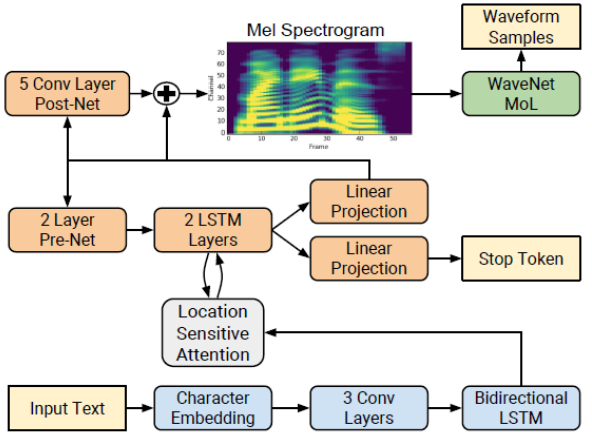
\includegraphics[width=0.6\textwidth]{tacotron2.png}
    \caption{Architecture of the Tacotron 2 model. Taken from the Tacotron 2 paper.}
    \label{fig:tacotron2}
\end{figure}

Benefits of Tacotron 2 include:
Tacotron 2, an end-to-end model, translates text directly into speech waveforms, removing the requirement for intermediary processes. It offers a complete text-to-speech synthesis solution.


Expressive and Natural Speech: Tacotron 2 produces speech that sounds expressive and natural. It produces high-quality synthesised speech by accurately capturing crucial features like intonation, rhythm, and pronunciation.
Tacotron 2 has a variety of speech qualities that can be customised, including accents, speaking style, and feelings. This adaptability makes it possible to produce speech that is customised for certain applications or user preferences.
Tacotron 2's drawback and limitations include:
Data Requirements: Training Tacotron 2 requires a significant amount of paired text and speech data.
Challenges with Uncommon Words and Context: It may face difficulties with uncommon words, pronouncing proper nouns, or understanding complex contextual information.
It can only take max 400 characters. If we provide more characters then the coherency reduces.
WaveGlow:
WaveGlow is another computer program that works with Tacotron 2. Its job is to convert the mel spectrograms created by Tacotron 2 into actual speech waveforms. WaveGlow uses a special technique to create high-quality speech sounds.
WaveGlow works by mapping the mel spectrograms to the speech waveforms. It does this using a series of mathematical operations. The end result is a speech waveform that sounds very similar to human speech.

\begin{figure}[htbp]
    \centering
    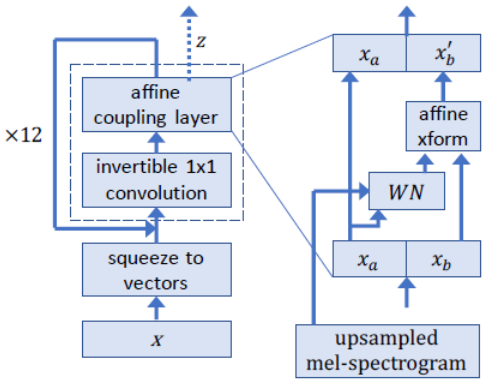
\includegraphics[width=0.6\textwidth]{waveglow.png}
    \caption{Architecture of the WaveGlow model. Taken from the WaveGlow paper.}
    \label{fig:waveglow}
\end{figure}

Benefits of WaveGlow
High-Quality Speech Synthesis: WaveGlow creates waveforms for speech that are of exceptional quality, catching minute details and resulting in realistic and natural-sounding speech.
WaveGlow produces speech waveforms in parallel, which makes it computationally more effective than models that produce samples one at a time.
Flexibility in Language and Voice: WaveGlow may be trained on a variety of datasets, allowing it to produce speech in a variety of languages and voices. It is not constrained to a particular tongue or vocalisation.

Limitations and Drawbacks of WaveGlow:
Tacotron 2 dependence: WaveGlow uses the mel spectrograms produced by Tacotron 2 as an input. Tacotron 2's output restrictions and flaws can have an impact on WaveGlow's ability to produce natural-sounding synthesised speech.
WaveGlow is a deep generative model, and as such, it calls for a lot of processing power, especially during the training stage. It could be necessary to use robust hardware or cloud infrastructure to implement and train WaveGlow.



% Methodology
\section{Methodology}
Describe your methodology in this section.

% Results
\section{Results}
Present your results in this section.

% Discussion
\section{Discussion}
Analyze and discuss your findings in this section.

% Conclusion
\section{Conclusion}
Summarize your work and provide conclusions.

% References
\bibliographystyle{plain}
\bibliography{references} % Replace "references" with the name of your .bib file

\end{document}